\documentclass{sintefbeamer}
\usepackage{amsfonts,amsmath,oldgerm}
%\usepackage{sidecap}
\usepackage{bm}
\usepackage{subfig}
\usepackage{stmaryrd}%\mapsfrom
\usepackage{graphbox} % allows includegraphics[align=c]

\newcommand{\mr}{\mathrm}
\newcommand{\mc}{\mathcal}
\let\SSS\S
\renewcommand{\S}{^\mr{S}}
\newcommand{\ii}{\mr{i}\,}
\newcommand{\ee}{\mr{e}}
%\newcommand{\phit}{\psi}
\newcommand{\phit}{\tilde\phi}
\newcommand{\br}[3]{\left#1#2\right#3}
\let\underscore\_
\renewcommand{\_}[1]{_\mr{#1}}
\newcommand{\oo}[1]{^{(#1)}}
\let\Re\relax
\let\Im\relax
\DeclareMathOperator\Re{Re}
\DeclareMathOperator\Im{Im}
\newcommand{\w}{w}
\newcommand{\ww}{\omega}
\newcommand{\zmap}{f}
\newcommand{\iJac}{|\zmap_\zz|^{-2}}


\newcommand{\bU}{\bm U}
\newcommand{\z}{z}
\newcommand{\x}{x}
\newcommand{\y}{y}
\newcommand{\zz}{\zeta}
\newcommand{\xx}{\xi}
\newcommand{\yy}{\sigma}
\newcommand{\h}{\hat}
\newcommand{\rbr}[1]{\left(#1\right)}
\newcommand{\sbr}[1]{\left[#1\right]}
\newcommand{\cbr}[1]{\left\{#1\right\}}

\newcommand{\testcolor}[1]{\colorbox{#1}{\textcolor{#1}{test}} \texttt{#1}}
\usefonttheme[onlymath]{serif}
\newcommand{\hrefcol}[2]{\textcolor{cyan}{\href{#1}{#2}}}

\title{Current and bathymetry extensions of the Higher Order Spectral method}
%\subtitle{}
\author{\href{mailto:andreas.akselsen@sintef.no}{Andreas Holm Akselsen}}
\date{July 7, 2022}
%\titlebackground{} % removes background

% separate section slide
\AtBeginSection[]{
  \begin{frame}
  \vfill
  \centering
  \begin{beamercolorbox}[sep=8pt,center,shadow=true,rounded=true]{title}
    \usebeamerfont{title}\insertsectionhead\par%
  \end{beamercolorbox}
  \vfill
  \end{frame}
}

\begin{document}
\maketitle

\newcommand {\framedgraphic}[2] {
    \begin{frame}{#1}
        \begin{center}
            \includegraphics[width=\textwidth,height=0.8\textheight,keepaspectratio]{#2}
        \end{center}
    \end{frame}
}


\begin{frame}{Background}{Simulation needs}
\vspace{-.5cm}
\small
\begin{itemize}
	\item Need for quick numerical wave tanks alongside experiments---digital twins.
	\begin{itemize}
		\item Result validation
		\item Pre: Support during planning stages
		\item Post: Better understanding experimental findings
	\end{itemize}
	\item Need for decision making tools for the design of new basin laboratories
	\begin{itemize}
		\item Capability and capacity
		\item Bathymetry effects
		\item Beach design
		\item Effect of current system
	\end{itemize}
\end{itemize}
\vspace{2mm}
\includegraphics[width=.45\textwidth,align=t]{./oldOB.PNG}%
\includegraphics[width=.25\textwidth,align=t]{./oldFloorRamp.PNG}%
\includegraphics[width=.3\textwidth,align=t]{./oldBeachDrawing.png}%
\end{frame}


\begin{frame}{The Higher Order Spectral method}
\vspace{-1cm}
\begin{center}
\includegraphics[width=.5\framewidth]{HOS1.png}
\end{center}

Body of fluid represented analytically:
\begin{align*}
\nabla^2\phi = 0;\qquad  \phi(x,y,t) = \sum_{j=1}^N \hat\phi_j(t) \frac{\cosh k_j(y+h)}{\cosh k_j h} \ee^{\ii k_j x}.
\end{align*}

We solve only the equations for the free surface 
\begin{align*}
h_t &=   - \nabla\eta\cdot\nabla\phi\S     + \big(1+|\nabla\eta|^2\big)(\phi_y)_{y=h}, %(\Phi_y)_{y=\eta} 
\\
\phi\S_t &= - \frac12\big|\nabla\phi\S|^2 + \frac12\big(1+|\nabla\eta|^2\big)(\phi_y)_{y=h}^2 - gh.
\end{align*}
with an ODE solver and match the modes $\hat\phi_j(t) $ to the surface potential $\phi\S(\bm r,t)$.
\end{frame}


\section{Representing a background flow field in HOS}

\begin{frame}{Adding a `background' potential}
	\vspace{-5mm}
	Adding a  pre-determined background potential $\Phi$
	\begin{align*}
		\tilde\phi = \phi + \Phi
	\end{align*}
	results in the boundary conditions
	\begin{align*}
		h_t &=   - \nabla\eta\cdot\nabla(\phi\S +\Phi)  + \big(1+|\nabla\eta|^2\big)\phi_y + \Phi_y,
		\\
		\phi\S_t &= -\Phi_t\big|_{y=\eta} - \frac12\big|\nabla(\phi\S +\Phi)|^2 + \frac12\big(1+|\nabla\eta|^2\big)\phi_y^2 - g h
	\end{align*}
	at $y=h(x,t)$.
	$\Phi$ can correct for the presence of a wavemaker, bathymetry alterations, \textit{a flow field}, etc. \\
	
	Myriad background flow fields can be constructed using classical (undergrad) potential theory.	
\end{frame}


\begin{frame}{Example: Steady fluid sources, sinks, vortices, doublets}
	Condition: Flow parallel to reference plane ($\sim$surface) and bathymetry + horizontally periodic or parallel to walls.\\
	$z=x+\ii y$, $w=\Phi + \ii\Psi$;
	\begin{equation*}
		W(z) =  U_0 z + \sum_j \sum_{n,m=-\infty}^{\infty} W_j(z + L n + \ii H m)
	\end{equation*}
	%	We require the uniform current $U\_{c}$ to be real (horizontal) and mirror each element $f_j$ about the plane $y=0$ by adding the conjugate element $f_j^*(\zeta^*)$ such that no streamlines crosses the plane $y=0$.
	%	Sources, sinks line vortices and doublets are used as flow elements: 
	with
	\begin{align*}
		W_j(z) &= 
		\begin{cases}
			A_j\ln(z-z_j) + A_j^*\ln(z-z_j^*) & \text{if element $j$ is source/sink/vortex,}\\
			-A_j/(z-z_j)-A_j^*/(z-z_j^*) & \text{if element $j$ is doublet.}
		\end{cases}
	\end{align*}
\end{frame}

\begin{frame}{Example: Waves propagating over a horizontal line vortex}
\centering
\vspace{-.25cm}
\begin{minipage}{.5\framewidth}
\includegraphics[width=\columnwidth]{../doc/figures/flowField_vortex.pdf}%
\end{minipage}%
\includegraphics[width=.5\framewidth,align=c]{../doc/figures/waveField_vortex.pdf}%
\end{frame}



\begin{frame}{Example: effect of a recirculation patch}
\vspace{-1cm}
\footnotesize
%\begin{minipage}{.5\framewidth}
\begin{align*}
W(z) &= U_0 z + \sum_{j=1}^\infty \hat\Phi_j \ee^{-k_jz},& % \quad k_j>0
\hat\Phi_j &= -\frac{\Gamma(k_j)}{\frac12 k_j h + \frac14\sin2k_jh},&
\Gamma(k) &= \int_{-h}^0 \!U\_I(y)\cos(k y)\,\mr d y.
\end{align*}
\begin{equation*}
%	{\tiny
%\begin{tabular}{c|ccc}
%	& Uniform & Linear & Flip-linear \\\hline
%	$U\_I(y)/\tilde U\_I$ & 
%	$\mc H(y) $&
%	$\frac{h+y}{h-d}\mc H(y)$&
%	$-\frac{d+y}{h-d}\mc H(y)$\\
%	$\Gamma(k)/\tilde U\_I$&
%	$-\frac{\sin kd}k$&
%	$\frac{\cos kd-\cos kh -k(h-d)\sin kd}{k^2(h-d)}$ &
%	$\frac{\cos kh-\cos kd }{k^2(h-d)}$\\
%	$U_0/\tilde U\_I$ &
%	$1-\frac hd$ &
%	$\frac12(1-\frac hd)$ &
%	$\frac12(1-\frac hd)$
%\end{tabular}
%}
\end{equation*}

\begin{center}
	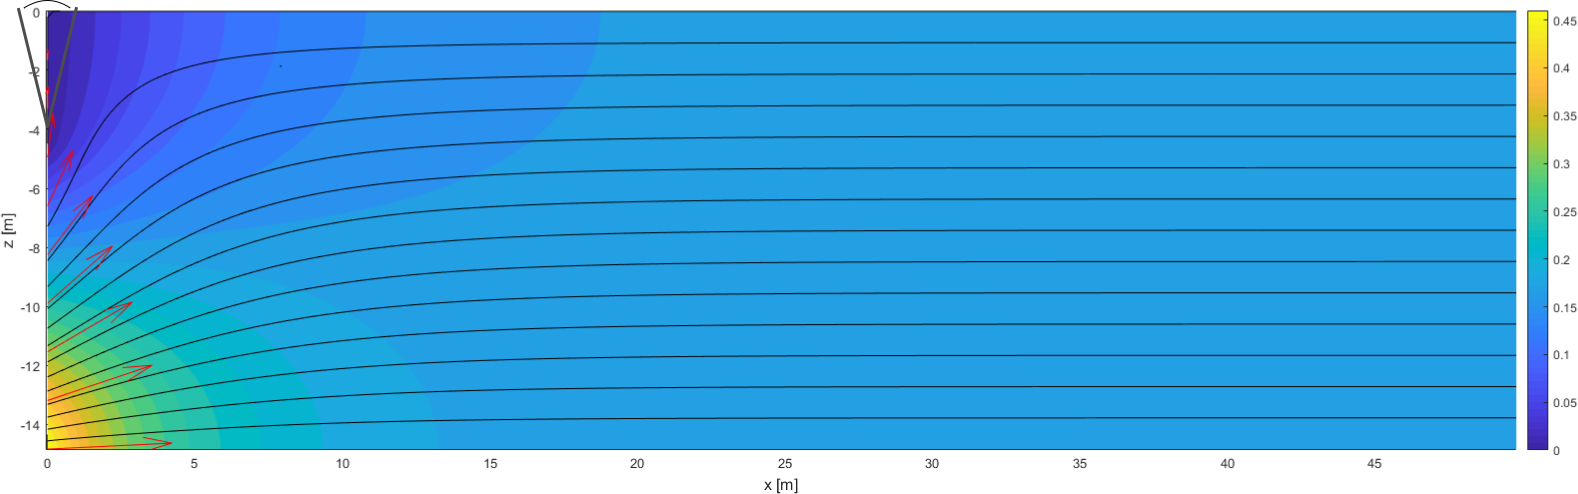
\includegraphics[width=.7\columnwidth]{currNoVortexBM.png}\\
	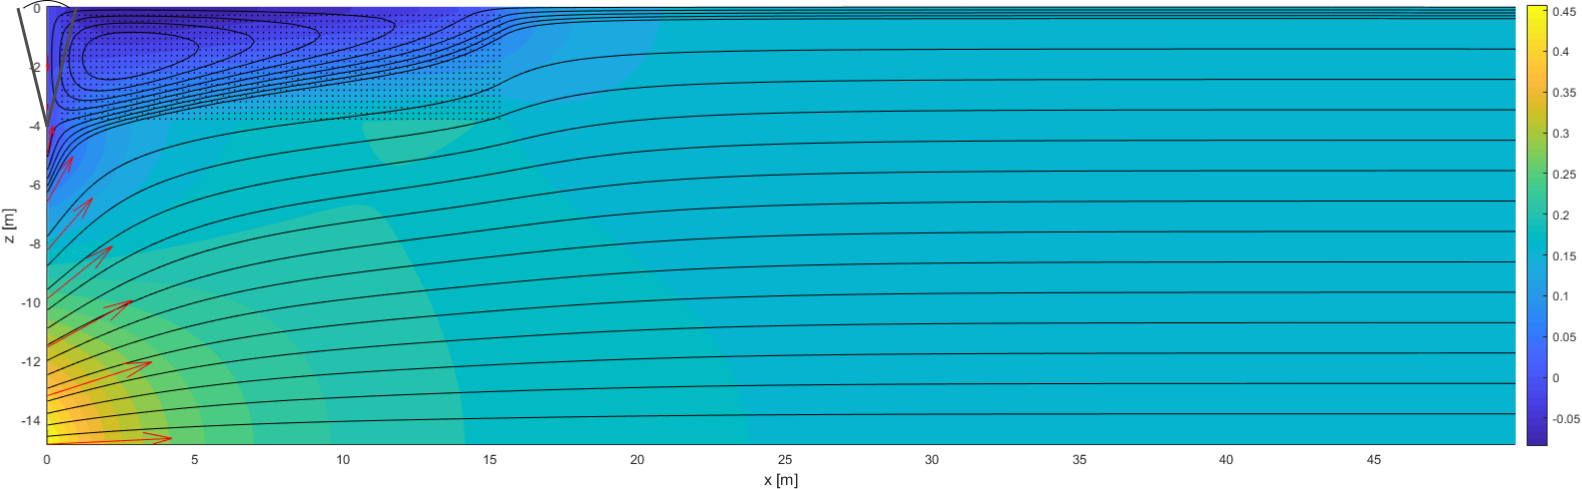
\includegraphics[width=.7\columnwidth]{currVortexBM.png}%
\end{center}
\end{frame}


\begin{frame}{Example: effect of a recirculation patch}
	\vspace{-5mm}
	\centering
	\includegraphics[width=.5\framewidth,align=c]{C:/gits/SFo_gitHOS/hosm-nwt2d/results/merged/snapCompare_T1p5CM2.pdf}\\
	$T=1.5$\,s
\end{frame}

%%%%%%%%%%%%%%%%%%%%%%%%%%%%%%%%%%%%%%%%%%%%%%%%

\section{Accounting for abrupt  bathymetry variation with conformal mapping}



\begin{frame}{Conformal mapping}
	\vspace{-5mm}
\centering
	%\includegraphics[width=.5\framewidth]{map.png}
	\includegraphics[width=.22\framewidth]{220px-Conformal_map.svg.png}
	\hspace{2cm}
	\includegraphics[width=.22\framewidth]{1200px-Biholomorphism_illustration.svg.png}\\
	
	Conformal  $\longrightarrow$  solution of Laplace equation in one plane implies solution in the other.\\
	 $\longrightarrow$ Analytic representation of $\phi$ remains valid in all planes.
\end{frame}

%%%%%%%%%%%%%%%%%%%%%%%%%%%%%%%%%%%%%%%%%%%%%%%%%


\begin{frame}{Conformally mapping bathymetry}{Schwartz--Christoffel transform}
	\vspace{-10mm}
	
	\[	\z\mapsfrom\zmap(\zz) \]
	\footnotesize
	 The Schwartz--Christoffel
	\begin{align*}
		\zmap'(\zz) &= C \prod_{j=1}^J (\zz-\xx_j)^{-\alpha_j/\pi},\\
		\intertext{yields}
		\zmap(\zz) &= \frac {H\_d-H\_s}\pi \left[  \sqrt{\zz-1}\sqrt{\zz+1} - 2\sinh^{-1}\! \sqrt{(\zz-1)/2} \right] - \ii H\_s.
	\end{align*}
\small
	\begin{center}
		\parbox[b]{.4\columnwidth}{\centering\includegraphics[width=.4\columnwidth]{../conformalMapping/conformalBathymetry/SC_step.pdf}\\$\z$-plane}%
		\qquad
		\parbox[b]{.4\columnwidth}{\centering\includegraphics[width=.4\columnwidth]{../conformalMapping/conformalBathymetry/SC_step_inv.pdf}\\$\zz$-plane}%
\end{center}
\end{frame}

\begin{frame}{Conformally mapping bathymetry}{Textbook example: duct expansion (\texttt{Milne-Thomson, 1967})}
	\vspace{-5mm}
\includegraphics[width=.33\textwidth]{./CCMei1.PNG}%
\includegraphics[width=.33\textwidth]{./CCMei2.PNG}%
\includegraphics[width=.33\textwidth]{./CCMei3.PNG}\\
	\vspace{3mm}
Let the streamlines themselves constitute a conformal map:
\small
\begin{align*}
	\lambda &= \exp(\zz),&
	\tau &= \sqrt{\frac{\lambda+c^2}{\lambda+1} },&
	f(\zz) = -\ii H\_s +\frac{H\_d}{\pi}\left[\frac1c \ln^+\frac{\tau-c}{\tau+c} - \ln\frac{\tau-1}{\tau+1}\right].
\end{align*}%
\begin{center}
	\parbox[b]{.4\framewidth}{\centering
		\includegraphics[width=.4\framewidth]{../conformalMapping/conformalBathymetry/CCMei_step.pdf}
		$\z$-plane
	}
	%\hfill$\rightarrow$ \hfill
	\qquad
	\parbox[b]{.4\framewidth}{\centering
		\includegraphics[width=.4\framewidth]{../conformalMapping/conformalBathymetry/CCMei_step_inv.pdf}
		$\zz$-plane
	}  
\end{center}
\end{frame}




%%%%%%%%%%%%%%%%%%%%%%%%%%%%%%%%%%%%%%%%%%%

\begin{frame}{Conformally mapping bathymetry}{Slope depth transitions}
\vspace{-1cm}
\small
\begin{equation*}
f'(\zz) \mapsfrom K \prod_{j=1}^{N_\angle} \rbr{\frac{\exp(\zz-\xi^\angle_j)+1}{\exp(\zz-\xx^\angle_j) + (H_{j+1}/H_j)^{\pi/\theta_j}}}^{\theta_j/\pi}
\end{equation*}
can be integrated numerically prior to simulation:

\includegraphics[width=.45\framewidth,align=c]{../conformalMapping/conformalBathymetry/SCnumStep2x45deg_zz.pdf}
$\rightarrow$
\includegraphics[width=.45\framewidth,align=c]{../conformalMapping/conformalBathymetry/SCnumStep2x45deg_z.pdf}
\\


\includegraphics[width=.45\framewidth,align=c]{../conformalMapping/conformalBathymetry/SCnumStepMulti_zz.pdf}
$\rightarrow$
\includegraphics[width=.45\framewidth,align=c]{../conformalMapping/conformalBathymetry/SCnumStepMulti_z.pdf}

\end{frame}



\begin{frame}{Boundary equations for $\zz$-variables}
\vspace{-.5cm}
\begin{align*}
	\zz &= \xx+\ii\yy, &
	\x+\ii h(\x,t) &\mapsfrom f[\xx+\ii \eta(\xx,t)], &
	 \varphi &= \Re w[f(\zz)];\; w(\z)=\phi+\ii\psi
\end{align*}
\begin{align*}
\eta_t &= \iJac\sbr{\varphi_\yy\rbr{1+\eta_\xx^2}-\varphi\S_\xx} + \eta_\xx \Re\rbr{\frac{\zmap_t}{\zmap_\zz}}-\Im\rbr{\frac{\zmap_t}{\zmap_\zz}},\\
\varphi\S_t &= - \frac12\iJac\sbr{\rbr{\varphi\S_\xx}^2-\rbr{1+\eta_\xx^2}\varphi_\yy^2} - gh + \varphi\S_\xx \Re\rbr{ \frac{\zmap_t}{\zmap_\zz}}.
\end{align*}
Usually, $f_t\equiv 0$.
\end{frame}
%



%%%%%%%%%%%%%%%%%%


\begin{frame}{Bathymetry step; $H\_d = 1.0$, $H\_s = 0.5$}
		\vspace{-5mm}
	\centering
	\parbox[b]{.5\columnwidth}{\centering \includegraphics[width=.45\columnwidth]{../HOS_bathymetry/figures/map/map_logstrip_SSGW_ka0p05_H1p00_0p50_Nw60.pdf}\\Full domain.}%
	\qquad
	\parbox[b]{.5\columnwidth}{\centering \includegraphics[width=.45\columnwidth]{../HOS_bathymetry/figures/map/mapZoom_logstrip_SSGW_ka0p05_H1p00_0p50_Nw60.pdf}\\Corner, 1--to--1.}
\end{frame}

\begin{frame}{Bathymetry step; surface elevation}
		\vspace{-5mm}
	\centering
	\includegraphics[width=.65\columnwidth]{../HOS_bathymetry/figures/logstrip_SSGW_ka0p05_M5_H1p00_0p75_Nw60_dt5T_nx3840_pad0_ikCutInf_Md0p5_r0p25.pdf}\\
	 $H\_s/H\_d = 0.75$.
\end{frame}

\begin{frame}{Bathymetry step; surface elevation}
		\vspace{-5mm}
	\centering
	\includegraphics[width=.65\columnwidth]{../HOS_bathymetry/figures/logstrip_SSGW_ka0p05_M5_H1p00_0p50_Nw60_dt5T_nx3840_pad0_ikCutInf_Md0p5_r0p25.pdf}\\
	$H\_s/H\_d = 0.50$.
\end{frame}

\begin{frame}{Bathymetry step; surface elevation}
		\vspace{-5mm}
	\centering
	\includegraphics[width=.65\columnwidth]{../HOS_bathymetry/figures/logstrip_SSGW_ka0p05_M5_H1p00_0p35_Nw60_dt5T_nx3840_pad0_ikCutInf_Md0p5_r0p25.pdf}\\
	$H\_s/H\_d = 0.35$.
\end{frame}

\begin{frame}{Results compared to linear and second-order theory Li \textit{et.\ al.} (2021)}
	\vspace{-5mm}
	\centering
	\includegraphics[width=.9\columnwidth]{../HOS_bathymetry/linearStepTheory/contourPlot.pdf}\\
%    \includegraphics[width=.3\columnwidth]{../HOS_bathymetry/linearStepTheory/R0.pdf}%
%	\includegraphics[width=.3\columnwidth]{../HOS_bathymetry/linearStepTheory/R0_k.pdf}%
	\small
	\begin{tabular}{c|ccc}
		$H\_s/H\_d$ & 0.75 & 0.50 & 0.35\\\hline
		$R_0$ & 0.054 & 0.135 & 0.208 \\
		$R\_{HOS}^{(1)}$ &  0.052 & 0.132 & 0.20\\\hline
		$T_{20}$ & 1.93 & 7.57& 18.58 \\
		$T^{(2)}\_{HOS}$ & 1.6 & 6.32 & 14.4
	\end{tabular}
\vspace{5mm}
\begin{flushleft}
	\texttt{ \scriptsize Y. Li, Y. Zheng, Z. Lin, T.A.A. Adcock;Surface wavepackets subject to an abrupt depth change. part 1. second-order theory. J.\ Fluid Mech., 915:A71, 2021}
\end{flushleft}
\end{frame}




%%%%%%%%%%%%%%%%%%%%%%%%%%

\begin{frame}{Comparing ramp slopes}
\begin{figure}%
\subfloat[$\theta=45$\textdegree]{\includegraphics[width=.33\framewidth]{../HOS_bathymetry/figures/map/mapZoom_SSGW_ka0p05_H1p00_0p50_nH2_ang1_0p5_Nw60.pdf}}%
\subfloat[$\theta=9$\textdegree]{\includegraphics[width=.33\framewidth]{../HOS_bathymetry/figures/map/mapZoom_SSGW_ka0p05_H1p00_0p50_nH2_ang1_0p1_Nw60.pdf}}%
\subfloat[$\theta=4.5$\textdegree]{\includegraphics[width=.33\framewidth]{../HOS_bathymetry/figures/map/mapZoom_SSGW_ka0p05_H1p00_0p50_nH2_ang1_0p05_Nw60.pdf}}%
\caption{Depth transition maps}
\end{figure}
\end{frame}


\begin{frame}{Step bathymetry, $H\_s/H\_d = 0.50$.}
\centering 
\vspace{-1cm}
\includegraphics[width=.75\framewidth]{../HOS_bathymetry/figures/logstrip_SSGW_ka0p05_M5_H1p00_0p50_Nw60_dt5T_nx3840_pad0_ikCutInf_Md0p5_r0p25.pdf}%
\end{frame}

\begin{frame}{45\textdegree{} slope depth transition.}
\centering
\vspace{-1cm}
 \includegraphics[width=.75\framewidth]{../HOS_bathymetry/figures/SSGW_ka0p05_M5_H1p00_0p50_nH2_ang1_0p5_Nw60_dt5T_nx3840_pad0_ikCutInf_Md0p5_r0p25.pdf}%
%\caption{Surface elevation, $(ka)_0 = 0.05$, $(kH)_0 = 1.00$ ($H\_d=1.0$\,m corresponds to $T\approx2.30$\,s); single slope with $\theta=\pi/4$; $H\_s/H\_d = 0.5$. Dashed lines indicate $\x$-location of slope transition beginning and end.}%
\end{frame}

\begin{frame}{9\textdegree{} slope depth transition.}
\centering
\vspace{-1cm}
 \includegraphics[width=.75\framewidth]{../HOS_bathymetry/figures/SSGW_ka0p05_M5_H1p00_0p50_nH2_ang1_0p1_Nw60_dt5T_nx3840_pad0_ikCutInf_Md0p5_r0p25.pdf}%
%\caption{Similar to \autoref{fig:res:slope1}, but with $\theta=\pi/20$.}%
\end{frame}

\begin{frame}{4.5 \textdegree{} slope depth transition.}
\centering
\vspace{-1cm}
 \includegraphics[width=.75\framewidth]{../HOS_bathymetry/figures/SSGW_ka0p05_M5_H1p00_0p50_nH2_ang1_0p05_Nw60_dt5T_nx3840_pad0_ikCutInf_Md0p5_r0p25.pdf}%
%\caption{Similar to \autoref{fig:res:slope1}, but with $\theta=\pi/40$.}%
\end{frame} 


\begin{frame}{Testing effect of beach extensions}
	\begin{figure}[H]
		\vspace{-1cm}
		\begin{minipage}[c]{.45\textwidth}\centering
		\includegraphics[width=\textwidth,align=c]{../conformalMapping/conformalBathymetry/beachRamp_h10D4th90_z.pdf}\\
		No beach extension
		\end{minipage}%
		\hfill
		\begin{minipage}[c]{.5\textwidth}\centering
			\includegraphics[width=1\textwidth]{../conformalMapping/conformalBathymetry/beachRamp_h10D4th45_z.pdf}\\
			$\theta=45$\textdegree{} beach extension.\\
			\includegraphics[width=1\textwidth]{../conformalMapping/conformalBathymetry/beachRamp_h10D4th30_z.pdf}\label{fig:map:30}\\
			$\theta=30$\textdegree{} beach extension.
		\end{minipage}
%		\subfloat[$\zz$-plane of map in \protect\subref{fig:map:30} ]{\includegraphics[width=.7\textwidth]{../conformalMapping/conformalBathymetry/beachRamp_h10D4th30_zz.pdf}}%
%		\caption{Bathymetries and conformal maps. Dashed line indicates the Lader tank beach profile $\y=-D(\x/L)^2$; $D/L=0.353$.}
		\label{fig:maps}
	\end{figure}
\end{frame}


\begin{frame}{	No beach extension, 2.50 second period.}
	\centering
	\vspace{-5mm}
	\includegraphics[width=.7\framewidth]{../HOS_bathymetry/figures/beach_SSGW_T2p50_ka0p05_M5_H10p00_2p00_theta90_Nw60_dt5T_nx3840_pad0_ikCutInf_Md0p5_r0p25_a10p0777_aRef0p00314.pdf}\\
\end{frame}

\begin{frame}{	$\theta=45$\textdegree{} beach extension, 2.50 second period.}
	\centering
	\vspace{-5mm}
	\includegraphics[width=.7\framewidth]{../HOS_bathymetry/figures/beach_SSGW_T2p50_ka0p05_M5_H10p00_8p30_4p90_2p00_theta90_180_45_Nw60_dt5T_nx3840_pad0_ikCutInf_Md0p5_r0p25_a10p0777_aRef0p00155.pdf}\\
\end{frame}

\begin{frame}{$\theta=30$\textdegree{} beach extension, 2.50 second period.}
\centering
\vspace{-5mm}
	\includegraphics[width=.7\framewidth]{../HOS_bathymetry/figures/beach_SSGW_T2p50_ka0p05_M5_H10p00_9p10_4p60_2p00_theta90_180_30_Nw60_dt5T_nx3840_pad0_ikCutInf_Md0p5_r0p25_a10p0777_aRef0p00149.pdf}\\
\end{frame}






%%%%%%%%%%%%%%%%%%%%%%%%%%%%


\begin{frame}{Power spectra in front and after depth transition}{Depth transition from 3.0 to 0.5 meters. $T\_p=2.5$\,s, $H\_s=0.125$\,m.}
\vspace{-1cm}
\scriptsize
	\begin{figure}[h!ptb]%
	\centering
	\subfloat{%[Bathymetries]
		\includegraphics[width=.75\columnwidth]{./zmapsCrop.png}
	%\includegraphics[width=.2\columnwidth]{../HOS_bathymetry/figures/map/mapZoom_82100_linear_ka0_H3p00_0p50_theta90_Nw1.pdf}
	%\includegraphics[width=.2\columnwidth]{../HOS_bathymetry/figures/map/mapZoom_82000_linear_ka0_H3p00_0p50_theta45_Nw1.pdf}
	%\includegraphics[width=.2\columnwidth]{../HOS_bathymetry/figures/map/mapZoom_82100_linear_ka0_H3p00_0p50_theta15_Nw1.pdf}
	}\\[-4mm]%
\subfloat[$x=0.0$\,m.]{
	\includegraphics[width=.28\columnwidth]{../HOS_bathymetry/figures/powerSpec/82100/x_wp0.pdf}}%
\subfloat[$x=5.0$\,m.]{
	\includegraphics[width=.28\columnwidth]{../HOS_bathymetry/figures/powerSpec/82100/x_wp5.pdf}}%
\subfloat[$x=10.0$\,m.]{
	\includegraphics[width=.28\columnwidth]{../HOS_bathymetry/figures/powerSpec/82100/x_wp10.pdf}}\\[-4mm]%
\subfloat[$x=15.0$\,m.]{
	\includegraphics[width=.28\columnwidth]{../HOS_bathymetry/figures/powerSpec/82100/x_wp15.pdf}}%
\subfloat[$x=20.0$\,m.]{
	\includegraphics[width=.28\columnwidth]{../HOS_bathymetry/figures/powerSpec/82100/x_wp20.pdf}}%
\subfloat[$x=25.0$\,m.]{
	\includegraphics[width=.28\columnwidth]{../HOS_bathymetry/figures/powerSpec/82100/x_wp25.pdf}}%
	\caption{}%Power spectra measured at various locations, comparing transitional ramps.
	%\label{fig:S}%
	\end{figure}
\end{frame}

\begin{frame}{Flat bottom reference}{Flat bed reference for depths 3.0 and 0.5 meters. $T\_p=2.5$\,s, $H\_s=0.125$\,m.}
%\vspace{-1cm}
\scriptsize
\begin{figure}[h!ptb]%
\centering
\subfloat[$x=0.0$\,m.]{
	\includegraphics[width=.28\columnwidth]{../HOS_bathymetry/figures/powerSpec/821x0_2xflatOnly/x_wp0.pdf}}%
\subfloat[$x=5.0$\,m.]{
	\includegraphics[width=.28\columnwidth]{../HOS_bathymetry/figures/powerSpec/821x0_2xflatOnly/x_wp5.pdf}}%
\subfloat[$x=10.0$\,m.]{
	\includegraphics[width=.28\columnwidth]{../HOS_bathymetry/figures/powerSpec/821x0_2xflatOnly/x_wp10.pdf}}\\[-4mm]%
\subfloat[$x=15.0$\,m.]{
	\includegraphics[width=.28\columnwidth]{../HOS_bathymetry/figures/powerSpec/821x0_2xflatOnly/x_wp15.pdf}}%
\subfloat[$x=20.0$\,m.]{
	\includegraphics[width=.28\columnwidth]{../HOS_bathymetry/figures/powerSpec/821x0_2xflatOnly/x_wp20.pdf}}%
\subfloat[$x=25.0$\,m.]{
	\includegraphics[width=.28\columnwidth]{../HOS_bathymetry/figures/powerSpec/821x0_2xflatOnly/x_wp25.pdf}}%
\caption{Flat bed reference.}
\end{figure}
\end{frame}








%%%%%%%%%%%%%%%%%%%%%%%%%%%%%%%%%%%%%%%%%%%%%%%%%%%%%%

\section{Conformally mapping the free surface itself}

\begin{frame}{Conformally mapped free surface}
\centering
\vspace{-1cm}
\small
\begin{align*}
\z \mapsfrom f(\zz) &= \sum_{j=-M}^M \h f_j \,\frac{\ee^{\ii k_j(\zz+\ii H)}}{\cosh(k_j H)}
&
\z \mapsfrom f(\zz) &= \sum_{j=-M}^M \h f_j \,\frac{-\ee^{\ii k_j(\zz+\ii H)}}{\sinh(k_j H)}.
 \end{align*}%
\normalsize

\includegraphics[width=.8\framewidth]{../HOS_old/conformalHOS/figures/imagedecayingConformalka0p2_M5_h1p00_Nw1_dt0p25T_nx512.pdf}%
\end{frame}

\begin{frame}{Conformally mapped free surface}
	\centering
%\vspace{-.5cm}
\includegraphics[width=.6\framewidth]{../HOS_ChalikovTaylor_current/figures/rounded2_contour.pdf}%



%\vspace{5mm}
\begin{flushleft}
	\texttt{ \scriptsize D. Chalikov and D. Sheinin. Modeling extreme waves based on equations of potential
		flow with a free surface. J.\ Comp. Phys., 210(1):247–273, 2005.}
\end{flushleft}

\end{frame}


%%%%%%%%%%%%%%%%%%%%%%%%%%%%%%%%%%%%%%%%%%%%%%%%%%%%%%

\section{Conformally mapping the wavemaker}

\begin{frame}{Representing a wavemaker with conformal mapping}
	\centering
\vspace{-1cm}
	\begin{equation*}
f_\zz(\zz,t) = \prod_{j=-\infty}^\infty \rbr{1+\frac{d^2}{\rbr{\zz+2\ii j h}^2}}^{\theta(t)/\pi}
= \sbr{1+\frac{\sin^2\!\frac{\pi d}{2h}}{\sinh^2\!\frac{\pi \zz}{2h}}}^{\theta(t)/\pi}
\end{equation*}

\includegraphics[width=.5\framewidth]{../conformalMapping/conformalWavemaker/mapFlap3_positive.pdf}%
\includegraphics[width=.5\framewidth]{../conformalMapping/conformalWavemaker/mapFlap3_negative.pdf}%
\end{frame}


\begin{frame}{Forward\ldots}
	\begin{itemize}
		\item Development
		\begin{itemize}
			\item Further validation.
			\item Wave breaking model.
			\item Improved wavemaker? 
			\item Combination of bathymetry and surface mapping?
			\item 3D?
		\end{itemize}
	\item Utilization
		\begin{itemize}
			\item Parametric design studies OSC.
			\item Digital twin in SINTEF projects.
			\item Grants, research \& publication.
		\end{itemize} 
	\end{itemize}

\end{frame}



\backmatter

\end{document}